%%
% 引言或背景
% 引言是论文正文的开端,应包括毕业论文选题的背景、目的和意义;对国内外研究现状和相关领域中已有的研究成果的简要评述;介绍本项研究工作研究设想、研究方法或实验设计、理论依据或实验基础;涉及范围和预期结果等。要求言简意赅,注意不要与摘要雷同或成为摘要的注解。
\chapter{绪论}
\label{chapter1: introduction}
%定义，过去的研究和现在的研究，意义，与现有结论的区别

\section{绪论}
\label{sec:background}
% What is the problem
% why is it interesting and important
% Why is it hards, why do naive approaches fails
% why hasn't it been solved before
% what are the key components of my approach and results, also include any specific limitations，do not repeat the abstract
%contribution
%引言是论文正文的开端，应包括毕业论文选题的背景、目的和意义；对国内外研究现状和相关领域中已有的研究成果的简要评述；创新点；介绍本项研究工作研究设想、研究方法或实验设计、理论依据或实验基础；涉及范围和预期结果等。要求言简意赅，注意不要与摘要雷同或成为摘要的注解。

\subsection{选题背景}


第五代移动通信系统（5G）已经大规模商用，在推动我国经济高质量发展、提升产业水平和服务群众生活中发挥了重要作用。然而，随着海量智能终端的普及以及网络化，社会工业生产对移动通信的需求不断增长，全新的应用场景不断涌现，5G 将难以满足未来通信需求。关于超五代 (Beyond 5G, B5G) 通信网络关键技术的研究正当其时。B5G 关键技术的研发需要响应不同业务场景的需求。作为 5G/B5G/6G 的重要业务场景，在当前的5G及即将到来的B5G（Beyond 5G）场景下，物联网（IoT）技术实现了更广泛的应用，成为智能互联设备与环境的核心驱动力。5G网络凭借高带宽、低延迟、超高可靠性和大规模连接能力，显著提升了物联网设备的连接效率，为各行业的数字化转型铺平了道路。海量机器型通信（massive Machine Type communications，mMTC）是指通过在机器上安装各种传感器和控制器等器件，来赋予机器智能的属性，使得机器与机器间能在无人控制的情况下，自主的进行数据交互的技术。mMTC业务场景主要解决大规模设备连接的需求，涵盖众多物联网新兴产业，比如数字低空产业、智慧港口和智慧医疗等，均为《2024 年广东省数字经济工作要点》中所指明的广东省重点发展领域。2023 年，mMTC 也被国际电信联盟无线通信部门（Radio Communication Division of the International Telecommunication Union， ITU-R）纳入 6G 业务愿景。因此，展开针对物联网业务场景的 B5G 关键技术研发对信息技术产业发展具有重要现实意义。

与传统的以人为中心的通信（Human Type Communications, HTC）不同， mMTC 业务场景具有海量接入、零星/短包传输、电量极度受限和上行为主等新流量特征。针对业务流量新特征，NB-IoT、LTE-M 和 LoRaWAN 等新技术或者系统被提出。相比 HTC，针对 mMTC 所设计的不同通信系统虽然网络架构和硬件设计等方面存在显著差异，但共同特征是 MAC 层普遍采纳了免授权随机接入机制(Grant-Free Random Access, GFRA)。在蜂窝网络场景下，GFRA 与传统的授权随机接入（Grant-Based Random Access, GBRA）有本质区别。

\begin{itemize}
	\item GFRA是指设备间通过随机接入协议，分布式共享的时频资源，数据报文直接参与信道竞争。
	\item GBRA是指设备先通过随机接入过程与基站建立空口承载链路，然后基站运用集中式资源调度算法，分配独占的时频资源给设备传输数据。
\end{itemize}

相比GBRA，在GFRA中，基站无需获知设备数据流量特征的先验信息，利用统计复用效应，让不宽裕的时/频/码资源支撑大量潜在设备的接入需求；另一方面，由于基站不需要与每个设备建立空口承载链路，基站运算和空口信令交互开销被大幅降低。因此，GFRA已被纳入蜂窝网络标准体系，GFRA和GBRA将共存于5G/B5G/6G网络已成为业界共识。然而，随物联网业务种类愈发繁杂、流量特征和服务质量要求愈发差异化，从MAC层协议角度，5G现有的GFRA和GBRA协议越来越难以高效支撑各类物联网业务。



\subsection{研究目的及意义}
%4.总结需求并引出选题意义
针对不同物联网业务场景下的随机接入机制协议，业界和学术界围绕GFRA和GBRA展开了系统性的性能分析和对比工作。从数据传输资源的调度模式差异可以看出，采用分布式接入的GFRA适用于零星、小数据报文传输的mMTC业务场景；采用集中式控制的GBRA适用于吞吐量较大或者频繁传输数据的mMTC/HTC业务场景。\cite{bibid}从信令开销的角度，提出了GF RA和GBRA共存5G网络中的接入机制选择策略，阐明了关于数据流量特征或者服务质量要求的判决门限。然而，在有限选项中择优选取，仅能实现相对最优。当物联网流量特征处于接入机制判决门限周边的范围——即流量既非零星/短包传输，也非大吞吐/频繁传输的场景时，GFRA和GBRA均无法为物联网业务提供高效的通信服务。选择GFRA可能因数据流过于密集而导致随机接入信道严重拥堵；而GBRA则可能由于数据流量偏低，造成不必要的接入成本上升，资源浪费，能耗增加。为适应于复杂多变的物联网流量特征，亟需研发创新的MAC层接入机制，以填补现有方案的空白，优化整体网络性能。
现有5G免授权随机接入机制（GFRA）的一个关键缺陷就在于僵化的资源利用模式。以5G NR两步随机接入为例，其沿袭了时隙Aloha协议的思路。设备每个数据报文在每个时隙（或时频资源块）以一定概率传输。每次传输决策仅针对当前的时频资源、至多争用一个时频资源块。在零星小报文mMTC场景下，由于信道负载轻且设备报文少，上述模式有效、可行。如果有多个数据报文需要传输时，受制于资源利用模式和决策机制，设备需要多次决策、多次竞争，导致资源利用率低下，接入信令/能量开销过高。
在本课题的前期工作中发现，破除5G接入机制僵化的资源利用模式的一个简单、直接和有效的方法即是充分利用随机接入信道的短时可用性。大量的仿真统计结果表明，在现有GFRA体制下，由于全网设备传输行为的随机性，单个设备在占用信道一个时隙后，信道实际上会有一定的概率存在连续空闲的情况。充分利用信道的短时可用性能提高随机接入信道的利用率，使得蜂窝系统在不增加时/频/码资源、不变更物理层信号处理体制的前提下，容纳更多的物联网设备和数据，具有重要的理论和工程意义。

具体而言，本课题首先提出一种动态接入时长的免授权接入机制（Dynamic Time-GFRA, DT-GFRA）。在DT-GFRA中，物联网设备采用单次决策、连续传输的机制，即在任一时隙，以一定概率决定传输后，设备将以非独占的形式，在信道上持续传输，直至队列为空、或者因信道衰落、或者因其他节点发起传输而造成干扰中断。该机制预期将至少有如下优势:
\begin{itemize}
	\item 承接传统固定时长的免授权随机接入机制（Fixed Time-GFRA, FT-GFRA）优势，DT-GFRA也不需要设备与基站建立空口承载连接，有效降低信令开销和能耗。
	\item 相比FT-GFRA，DT-GFRA在接入策略上更加弹性和激进，以快速报文续传的模式，利用信道的短时可用性，有效提升网络容量。
	\item DT-GFRA从MAC层协议上创新，无须更改物理层设计，具有广泛的兼容性、实用性和可行性，为B5G网络接入机制设计带来重要理论启示和实现可能。
\end{itemize}

然而如同其他所有类型的随机接入协议，DT-GFRA协议下的网络性能与接入控制参数、资源配置参数等息息相关。为此，本课题将立足3GPP标准协议，围绕物联网业务场景，针对DT-GFRA机制，解决三个问题：如何分析、如何优化及如何实施。具体来说，本课题将重点研究在DT-GFRA机制下，业务流量特征参数和网络参数对MTC设备接入行为与信道占用状况影响机理；运用排队论，构建低复杂度、可优化Markov模型；在复杂物联网业务场景下，进一步引入强化学习算法，提升DT-GFRA的适用广度与能力；基于5G NR两步随机接入协议流程，从信令交互流程的角度，探讨DT-GFRA在蜂窝网络中的实施途径。
本课题旨在设计创新的DT-GFRA机制，突破传统FT-GFRA僵化的资源利用模式、提升网络能效，并构建从理论建模、性能优化到应用实施的完整的理论及技术方案，丰富B5G网络MAC层接入协议体系。


\section{国内外研究现状和相关工作}


作为蜂窝网络标准制定组织3GPP指定的5G三大业务场景之一，海量机器型通信（mMTC）已是学界和工业界研究的焦点。围绕物联网场景的接入机制研究，当前研究工作大致可以分为三类：（1）接入机制设计、（2）网络参数优化和（3）物理层改进。
\subsection{接入机制设计}

早在2010年，3GPP就启动了关于mMTC的接入网（Radio Access Network，RAN）改进项目，发布3GPP TR 37.868文档，阐述了RAN对mMTC业务承载能力的局限性，并围绕接入控制，提出了RAN改进的方向\cite{bibid}。对于4G LTE网络而言，其技术体系面向以人为中心的通信（Human Type Communications, HTC）进行设计，接入机制采用GBRA思想，其随机接入过程基于时隙Aloha协议，即用户节点在每个随机接入信道（Physical Random Access Channel, PRACH）时隙，独立的决定是否发送接入请求\cite{bibid}。由于PRACH资源有限，海量的mMTC接入请求将导致PRACH的严重拥塞和网络瘫痪。同时，mMTC接入后，往往仅传输少量的数据报文。建立空口承载所引发的信令/能耗开销超过数据报文传输量及效益，凸显了GBRA支撑mMTC的局限性\cite{bibid}。针对mMTC业务小数据报文传输的特征，3GPP在保留传统的GBRA的同时，为5G蜂窝网络引入固定时长的免授权随机接入机制（Fixed Time-GFRA, FT-GFRA），也就是四步/两步随机接入过长\cite{bibid}。GFRA制式下，设备在随机接入过程中就已经完成报文传输，不再额外需要搭建无线资源控制层（Radio Resource Control，RRC）资源连接，从而大大降低信令开销\cite{bibid}。目前GFRA被公认为是蜂窝网络支撑mMTC业务的主流范式。

除了以上由3GPP主导改进的接入机制，学者从整个蜂窝系统架构的角度提出更多新颖的策略。例如[10]-[12]提出多层汇聚接入机制，即mMTC设备首先通过非授权频段的Device-to-Device链路将数据报文汇聚至中心节点，然后再由中心节点与基站进行通信，以此大幅降低PRACH信道拥塞，提升单次接入所传输的数据量和能效。[13]-[16]设计了Tree-Splitting接入机制去灵活协调随机接入资源，即为每一个发生报文碰撞的PRACH时频资源块，调度额外的两至三个PRACH时频资源块，通过持续迭代，不断地降低单个PRACH时频资源块上的竞争用户量，直至确保每个用户成功接入。[17]-[19]考虑运用多种空口接入技术支撑mMTC业务，即除了5G蜂窝网络外，系统还可以利用其他的通信技术，例如低功耗广域网络通信技术和低轨卫星通信技术，通过增加空口接入技术冗余度，提升mMTC通信的可靠性。虽然仿真结果显示上述新颖的接入策略能明显提升蜂窝网络接入效率，但网络架构及通信协议需要大幅变更，短时内现实可行性低。

\subsection{网络参数优化}

基于给定的接入机制（包括授权接入或者是免授权接入），通过优化网络参数（包括时频资源、冲突退避和功率等）配置，提升随机接入效率是目前大部分学者所关注的主要研究方向。网络参数优化有两个重要的切入点：流量调度和资源调度。流量调度通过退避机制实现。退避参数主要是MAC层的Backoff窗口和RRC层的Access Class Barring因子。其本质都是让接入失败的UE回退一段随机的时长，再重新发起接入请求，以使海量的、突发的流量在时域上扩散平缓，降低单个时隙的接入请求数量，从而缓解拥塞。资源调度主要包括调度物理随机接入信道（Physical Random Access Channel, PRACH）的时频资源和随机接入前导序列码（Preamble）资源。为合理的调度流量和资源，针对接入性能优化，学者们提出了各种基于接入信道负载的流量调度和资源调度算法，比如根据信道环境，自适应的调整接入请求传输概率[20]、[21]、前导序列资源数目[22]-[24]，随机接入时隙资源数目[23]等。本课题组中立足3GPP MAC层标准协议，针对接入请求，构建了基于Markov状态转移的行为模型，探索了4G/5G网络随机接入信道的极限性能和最佳退避/资源参数的配置方案[25]-[27]。上述参数优化方法依赖于明确的数学模型，然而受限于复杂度，难以扩展至多业务场景或者是动态业务场景。
近年来，运用机器学习算法，特别是强化学习算法，动态优化网络参数，提升随机接入机制性能已成为研究热点。将每个设备视为一个独立的智能体，让其在每个时隙决定是否传输，是目前相关研究的主流切入点。在同构场景中，一些研究者将信道模拟为多信道结构，从频域方向解决相应的动态多信道接入问题。例如，[28]结合Q-Learning 和深度神经网络（Deep Neural Network，DNN）的方法，并提出了一种 DQN 模型。该模型以时间序列的历史观测为输入，通过预测近似的 Q 值, 指导用户如何在多信道环境中灵活切换，以优化频谱的使用。尽管如此，存在的局限性不容忽视。当涉及的信道数量增加时，模型的训练周期随之延长，这会导致实时性能下降，不利于应对快速变化的无线环境。此外，面对大规模的网络用户群体，所提方法依赖于一个集中式控制器来进行信道的分配和冲突管理。这个控制器在每个时间槽中负责选择一个最优的非正交信道子集，并为每个用户分配信道以避免潜在的信号冲突。然而，这种集中式计算策略不仅计算负荷重，而且可能需要大量的信令交互，带来了显著的通信开销，在大型或分布式网络的实际部署中仍需进一步优化以满足效率和可伸缩性的需求。近年，多智能体强化学习（Multi-Agent Reinforcement Learning，MARL）由于其解决高维决策问题以及快速收敛到协作策略的能力，被考虑应用于多址接入机制设计中。例如，[29]中采用 QMIX 算法设计的 QLBT（QMIX-advanced Listen-Before-Talk）多址接入机制，实现比 CSMA/CA 更高的吞吐量和更低的平均延迟，[30]基于多智能体深度确定性策略梯度（Multi-Agent Deep Deterministic Policy Gradient， MADDPG）算法提出了一种联合学习信道访问策略的多址接入机制，在吞吐量方面取得了良好的性能。[31]-[34]则围绕异构随机接入场景展开强化学习算法设计。课题团队在前期工作[35]提出了一种基于多智能体近端策略优化的新型MAC协议，通过在线多智能体强化学习，提升随机接入效率和公平性，同时减少通信开销。


\subsection{物理层改进技术}

通过引入massive MIMO、编码和非正交多址技术等物理层技术，提升系统容量，是目前学者们探索未来B5G/6G mMTC通信场景的一条重要技术路线。以非正交多址技术为案例，学者们分析了基于各类非正交多址接入技术的复杂接收机的性能，例如Gain Division Multiple Access (GDMA)[36], Sparse Code Multiple Access (SCMA)[37], Pattern Division Multiple Access (PDMA)[38]， Resource Spread Multiple Access (RSMA)[39] 和 Irregular Repetition Slotted Aloha [40]等。在[41]中，作者就基于经典的Bianchi模型分析了在非正交多址接入技术体系下，FT-GFRA的吞吐和时延性能，其结果显示非正交多址接入技术，相比传统的正交多址接入技术，可以大幅提升面向报文的随机接入机制。然而，非正交多址接入技术对系统信号处理能力和运算能力提出了较高的要求，不适用于以低功耗、低成本为特点的机器型通信网络，难以短期内在3GPP框架内实现应用落地。

\subsection{国内外文献分析小结}
综上所述，以提升免授权随机接入机制(Grant-Free Random Access, GFRA)性能为目标，现有文献在随机接入机制设计、网络参数优化方法和物理层改进技术等方面已经做了深入探索。然而，对极限接入性能的进一步提升往往伴随网络架构、协议体系和物理层收发信机的大幅改动，短时间内的现实可行性较低。如何在蜂窝系统框架下，通过3GPP协议扩展，设计创新性的接入机制，弥补传统固定时长的免授权随机接入机制（Fixed Time-GFRA, FT-GFRA）的缺陷，实现B5G网络对未来物联网业务的高效的支撑能力，仍是有待解决的问题。



\section{本文研究目标与内容}


\subsection{本文创新点与主要贡献}

本课题提出了一种新型的随机接入机制，即动态时长的免授权接入（DT-GFRA），并且以休假排队论以及多智能体强化学习算法为分析框架，在单/多业务场景条件下，揭示DT-GFRA的各项网络性能。此外，DT-GFRA可以很好兼容于现有的5GNRMAC层，不需要对物理层进行大幅度改动。预期创新点如下：
\begin{itemize}
\item[1.]
提出一种新型随机接入机制，即DT-GFRA。该机制可以很好兼容于现有5G NR的MAC标准，不需要大幅度改动物理层。

\item[2.]
利用休假排队模型构建对于DT-GFRA的分析框架，获得在饱和/不饱和场景下，吞吐/时延等网络指标的显式表达式。以指标表达式为基础，通过调整网络参数实现性能优化，并分析协议性能极限。

\item[3.]
利用多智能体强化学习算法，设计适应于DT-GFRA机制的强化学习框架。

\item[4.] 
能效为目标，给出现有FT-GFRA和GBRA，加上新提出的DT-GFRA三种机制在不同流量场景下的最优接入机制选择方案。

%到6G移动通信网络设计的灵活性和拓展性原则，以及
%在文献\cite{dai2012stabilitydelayofBA}的Aloha网络解析框架基础上创新性地引入了丢包机制。尽管在一定程度上对传输可靠性和能量效率造成了损失，但该机制的引入从建模层面增强了网络的时延性能表现。而重传限制$M$作为一个可调的系统参数，增加了通信系统的设计自由度，进而从性能优化层面增强了灵活性和拓展性。

\end{itemize}

\section{论文结构安排}
\label{sec:arrangement}
本文共分为六章，各章节内容安排如下：

第一章绪论。该章节系统详细地阐述了本文的选题背景意义、国内外研究现状和不足以及本文的创新点和贡献。

第二章系统建模。该章节首先给出通信网络所处的场景和假设。引入了基于吞吐量时延等概念，并给出了一种休假排队模型框架，为后续章节的分析提供基本分析视角。

第三章是基于ALoha的连续传输分析框架。

第四章是基于CSMA的连续传输分析框架。该章节在第二章建模的基础上推导出时延指标关于关键网络参数的闭式解。

第五章是实际通信系统的连续传输机制应用。该章节在前面两章基础上给出实际通信系统的应用。

第六章是本文的最后一章,总结与展望。是对本文内容的整体性总结以及对未来工作的预期。


%\begin{figure}[h]
%\centering 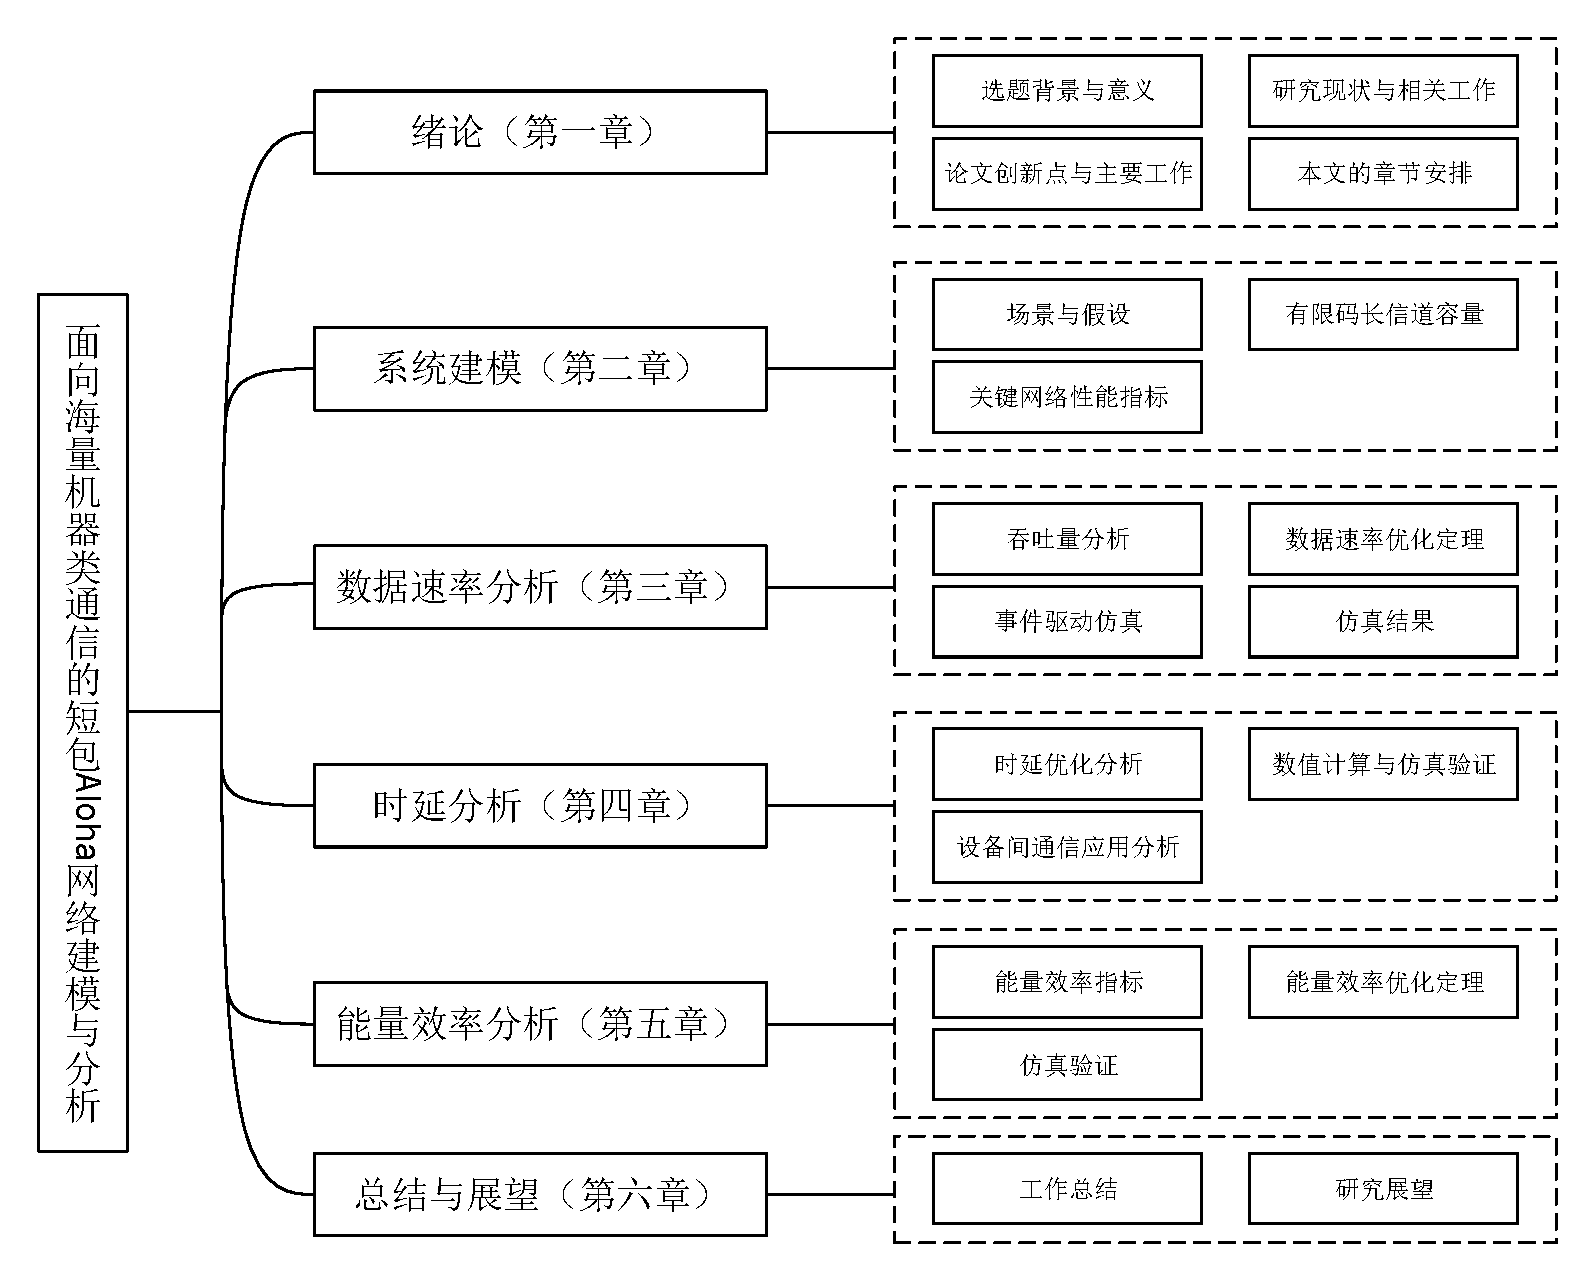
\includegraphics[angle=0,width=155mm,height=125mm]{image/weihua/structure.pdf}
%	\caption{论文章节安排}
%\label{fig:structure}
%\end{figure} 